\documentclass[12pt,a4paper,UTF8]{ctexart}
\usepackage{graphicx}
\usepackage{amsmath}
\usepackage{amssymb}
\usepackage{cite}
\usepackage[ntheorem]{empheq}
\usepackage{enumitem}
\usepackage{fullpage}
\usepackage{tocbibind}
\usepackage[bookmarksopen=true,colorlinks,linkcolor=black]{hyperref}
\usepackage{cellspace}
\usepackage{listings}
\usepackage{color}
\usepackage{epstopdf}
\usepackage{subfigure}
\usepackage{algorithm}
\usepackage{algorithmicx}
\usepackage{algpseudocode}

\renewcommand{\algorithmicrequire}{\textbf{Input:}}  % Use Input in the format of Algorithm
\renewcommand{\algorithmicensure}{\textbf{Output:}} % Use Output in the format of Algorithm

\usepackage{longtable}

\usepackage{float}
\definecolor{gray}{rgb}{0.5,0.5,0.5}
\definecolor{dkgreen}{rgb}{.068,.578,.068}
\definecolor{dkpurple}{rgb}{.320,.064,.680}

% set Matlab styles
\lstset{
   language=Matlab,
   keywords={break,case,catch,continue,else,elseif,end,for,function,
      global,if,otherwise,persistent,return,switch,try,while},
   basicstyle=\ttfamily,
   keywordstyle=\color{blue}\bfseries,
   commentstyle=\color{dkgreen},
   stringstyle=\color{dkpurple},
   backgroundcolor=\color{white},
   tabsize=4,
   showspaces=false,
   showstringspaces=false
}

\begin{document}
\CJKfamily{zhkai}	


\begin{center}
\textbf{作业三}\\
\textbf{姓名\quad 徐家恒~~~~~~~~~~~~~ 学号 PB18000334~~~~~~~~~~~~~~ 日期 2021.	6.16}\\
\end{center}

\begin{center}
\fbox{
\begin{minipage}{40em}
\vspace{5cm}
\hspace{20cm}
\end{minipage}}
\end{center}
\vspace{1cm}

\begin{enumerate}
	\item[第一题]
	本题考虑使用Richardson外推技术提高向前差商求给定函数导数的精度。

	(a) (5分)使用向前差分计算$f(x) = \sin(x)$在$x = 1.2$处的导数并使用loglog图
展示其精度随离散区间大小h的变化。h取$10^0, 10^{-1}, 10^{-2}, 10^{-3}, \dots, 10^{-15}$。\\

	代码如下:\\
\begin{lstlisting}[frame=single,numbers=left]
clc,close;

f = @(x) sin(x);
x0 = 1.2;

x1 = zeros(1, 16);
x2 = zeros(1, 16);
for i = 1 : 16
    x1(i) = 10^(1 - i);
    x2(i) = abs((f(x0 + x1(i)) - f(x0)) / x1(i) - cos(x0));
end

loglog(x1, x2)
\end{lstlisting}

	得到的精度如下图\ref{jpg:1}\\
	\begin{figure}[H]
		\centering
     	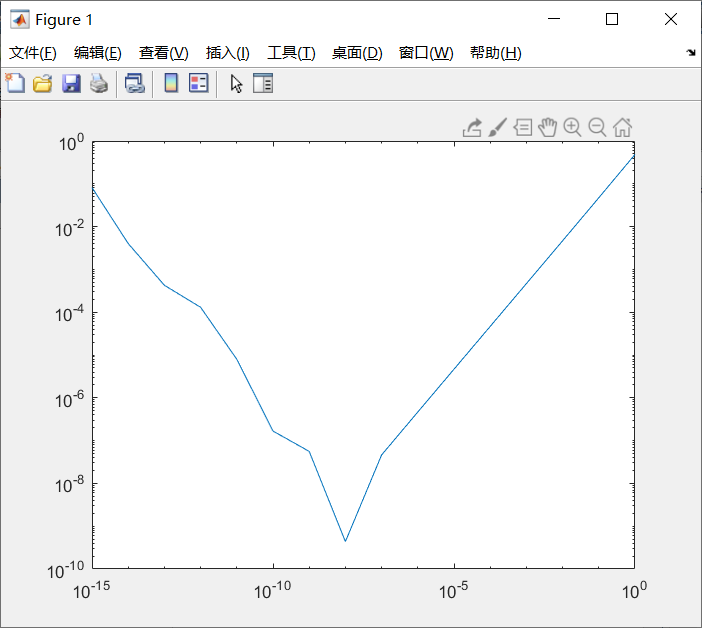
\includegraphics[width=0.8\textwidth]{1.png}
    	\caption{用向前差分计算导数的精度图像}\label{jpg:1}
	\end{figure}

	(b) (10分)推导出使用Richardson外推技术的向前差商的计算公式并用伪代码给出算法。\\

	由泰勒展开
$$f(x_0+h)=f(x_0)+h f^\prime (x_0) + \frac{h^2}{2!}f^{\prime \prime}(x_0)+O(h^2)$$ 
	得
$$f^\prime (x_0) = \frac 1 h (f(x_0 + h)-f(x_0))- \frac{h}{2}f^{\prime \prime}(x_0)+O(h)$$
	记
$$N_1 (h) = \frac{f(x_0 + h)-f(x_0)}{h}$$
\begin{equation}
f^\prime (x_0)=N_1(h)+c_1 h + O(h)
\label{eq:1}
\end{equation}
\begin{equation}
f^\prime (x_0)=N_1(\frac h 2)+c_1 (\frac h 2) + O(h)
\label{eq:2}
\end{equation}
	2·(\ref{eq:2})-(\ref{eq:1})
$$f^\prime(x_0)=\frac 1 {2-1} (2 N_1(\frac h 2)-N_1(h))+O(h)\approx N_2(h)$$
$$N_2(h)= N_1(\frac h 2) + \frac { N_1(\frac h 2)-N_1(h)}{2-1}$$
	继续外推下去,得到
$$N_{j}(h)=N_{j-1}(\frac{h}{2})+\frac{N_{j-1}(\frac{h}{2})-N_{j-1}(h)}{2^{j-1}-1}, \quad j=2,3, \cdots$$
$$f^\prime(x_0)=N_j(\frac h 2)+O(h^j)$$

	伪代码:\\
	
$let \quad A[1\dots maxrept] \quad a\quad  new\quad array$

$A[1] = N_1(h)$

$for \quad i = 1\quad to\quad maxrept$

$\quad tmp = A[1]$

$\quad for \quad j = i\quad to\quad 1\quad descend$

$\quad \quad A[j] = A[j+1]+(A[j+1]-A[j])/(2^{i-j+1}-1)$

$\quad end$

$\quad if \quad \lvert tmp - A[1] \rvert < \epsilon$

$\quad \quad return \quad tmp$

$\quad endif$

$end$

	(c) (5分)使用你的算法计算$f(x) = \sin(x)$在$x = 1.2$处的导数并使用semilogy图展示其精度随外推次数变化的情况。请自己选取h初始值,使得用外推方法能够算出的最精确的导数尽量精确。你的回答需要说明你使用外推方法算出的导数值是多少、误差又是多少、h的初始值是多少、外推了多少次。\\

	代码如下:\\
\begin{lstlisting}[frame=single,numbers=left]
clear,clc

syms x;
f = @(x) sin(x);
x0 = 1.2;
maxrept = 200;
tmp0 = cos(1.2);

B = ones(1, 11);
for k = 5 : 15
    epsilon = 10^(-k);
    maxp = 0;
    maxi = 0;
    for p = 0 : 15
        h = 10 ^ (-p);
        A = zeros(1, maxrept);
        A(1) = N1(f, x0, h);
        tmp1 = 0;
        for i = 1 : maxrept
            tmp1 = A(1);
            A(i + 1) = N1(f, x0, h / 2 ^ i);
            for j = i : -1 : 1
                A(j) = A(j + 1) + (A(j + 1) - A(j)) / (2 ^ (i - j + 1) - 1);
            end
            if abs(tmp1 - A(1)) < epsilon
                if abs(A(1) - tmp0) < abs(B(k - 4) - tmp0)
                    B(k - 4) = A(1);
                    maxp = p;
                    maxi = i;
                end
            end
        end
        if i == maxrept
            %fprintf('h : %e\texceed\n', h);
        end
    end
    fprintf('epsilon : %e\th : %e\ttimes : %d\tres : %.15f\terror : %e\n', 10^(-k), 10^(-maxp), maxi, B(k - 4), abs(B(k - 4) - tmp0));
end
semilogy(abs(B - tmp0))

function [res] = N1(f, x0, h)
    res = (f(x0 + h) - f(x0)) / h;
end
\end{lstlisting}

	结果:\\
\begin{lstlisting}[frame=single,numbers=left]
epsilon : 1.000000e-05	h : 1.000000e+00	times : 7	res : 0.362357754476673	error : 3.885781e-16
epsilon : 1.000000e-06	h : 1.000000e+00	times : 7	res : 0.362357754476673	error : 3.885781e-16
epsilon : 1.000000e-07	h : 1.000000e+00	times : 7	res : 0.362357754476673	error : 3.885781e-16
epsilon : 1.000000e-08	h : 1.000000e+00	times : 7	res : 0.362357754476673	error : 3.885781e-16
epsilon : 1.000000e-09	h : 1.000000e+00	times : 7	res : 0.362357754476673	error : 3.885781e-16
epsilon : 1.000000e-10	h : 1.000000e+00	times : 7	res : 0.362357754476673	error : 3.885781e-16
epsilon : 1.000000e-11	h : 1.000000e-01	times : 6	res : 0.362357754476665	error : 8.437695e-15
epsilon : 1.000000e-12	h : 1.000000e-01	times : 6	res : 0.362357754476665	error : 8.437695e-15
epsilon : 1.000000e-13	h : 1.000000e-01	times : 6	res : 0.362357754476665	error : 8.437695e-15
epsilon : 1.000000e-14	h : 1.000000e+00	times : 9	res : 0.362357754476749	error : 7.527312e-14
epsilon : 1.000000e-15	h : 1.000000e+00	times : 9	res : 0.362357754476749	error : 7.527312e-14
\end{lstlisting}

	得到的不同精度在最优h下得到的导数如下图\ref{jpg:2}\\
	\begin{figure}[H]
		\centering
     	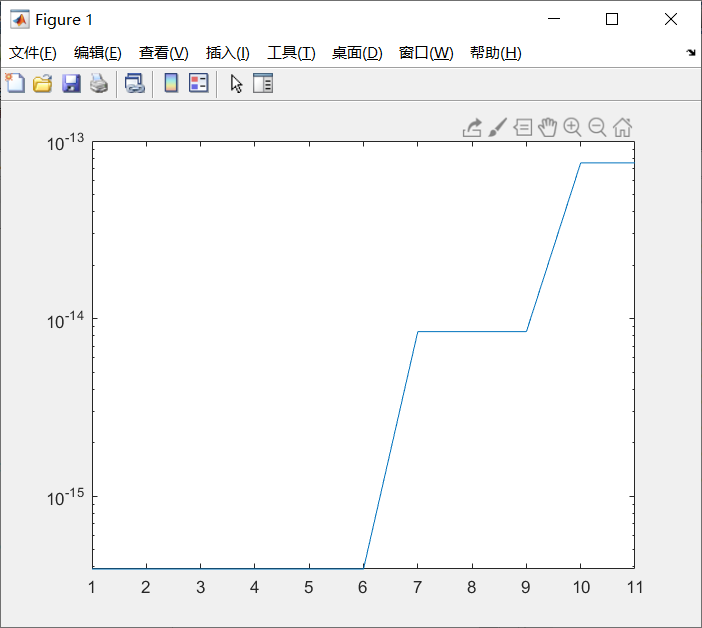
\includegraphics[width=0.8\textwidth]{2.png}
    	\caption{不同精度在最优h下得到的导数图像}\label{jpg:2}
	\end{figure}
	\item[第二题]
	本题讨论使用复化梯形公式求周期函数的积分。

	(a)(10分)证明当 $r$ 不是 $m$ 的整倍数的情况下,使用 $m$ 个子区间的复化梯形公式可以精确积分
$$\int_{-\pi}^{\pi} \cos (r x) d x  \text { 和 }  \int_{-\pi}^{\pi} \sin (r x) d x$$
     注意:这一结论类似于课堂上我们定义的代数精度。同时说明如果 $r$ 为 $m$ 的 整倍数时复化梯形公式对于上面两个积分会给出怎样的结果。

	记 $M_{2}=\max _{a \leqslant x \leqslant b}\left|f^{\prime \prime}(x)\right|$, 则
                    $$
                    \left|E_{n}(f)\right| \leqslant \frac{(b-a)^{3}}{12 n^{2}} M_{2}=O\left(\frac{1}{n^{2}}\right)
                    $$
                    对于任给的误差控制小量 $\varepsilon>0$,
                    $$
                    \frac{(b-a)^{3}}{12 n^{2}} M_{2}<\varepsilon \quad \text { 或 }\quad n \geqslant\left[\sqrt{\frac{(b-a)^{3} M_{2}}{12 \varepsilon}}\right]+1
                    $$
	就有 $\left|E_{n}(f)\right|<\varepsilon$,由
                    $$cos^{\prime \prime}(rx)=-r^{2}cos(rx),sin^{\prime \prime}(rx)=-r^{2}sin(rx)$$
                    得$M_{2}=r^{2}$,则$r$是$m$的整数倍时,有
                    $$
                    \frac{(2\pi)^{3}}{12 m^{2}}k^{2} m^{2}= \frac{(2\pi)^{3}}{12}k^{2} > \varepsilon
                    $$
无论如何都无法精确积分,$r$不是$m$的整数倍时,只需满足
                    $$m \geqslant\left[\sqrt{\frac{(2\pi)^{3} r^{2}}{12 \varepsilon}}\right]+1
$$便可使用$m$个子区间精确积分。
	

	(b)(10分)由于任意的以 $2 \pi$ 为周期的周期函数都可以表示为由正弦与余弦函数 的线性组合,所以上一问中所证明的定理实际上告诉我们求解一个周期函 数的积分的有效方法正是复化梯形公式。现使用复化梯形公式和不同数量 的子区间个数来求 $f(x)=e^{\cos (x)}$ 在 $[-\pi, \pi]$ 的积分,并用这个函数的真实积分 值作为参照使用semilogy图画出随着子区间数量 $m$ 变化所得到的积分精度 的变化。\\
                    题后语: 复化梯形公式之于周期函数的积分如同Gauss积分公式之于非周期
                    函数的基于多项式的积分。因此复化梯形公式是最有效的求解周期函数积分 的方法。

代码如下:\\
\begin{lstlisting}[frame=single,numbers=left]
clc,clear

f = @(x) exp(cos(x));
exact = 7.9549265210128452745132196653;

for i = 10 : 100
    step = 2 * pi / i;
    tmp = f(-pi)/2 + f(pi)/2;
    para = -pi + step;
    for j = 1 : i - 1
        tmp = tmp + f(para);
        para = para + step;
    end
    tmp = tmp * step;
    T(i - 9) = abs(tmp - exact);
end

semilogy(T)
\end{lstlisting}

得到的不同子区间数量下计算面积的误差如下图\ref{jpg:3}\\
	\begin{figure}[H]
		\centering
     	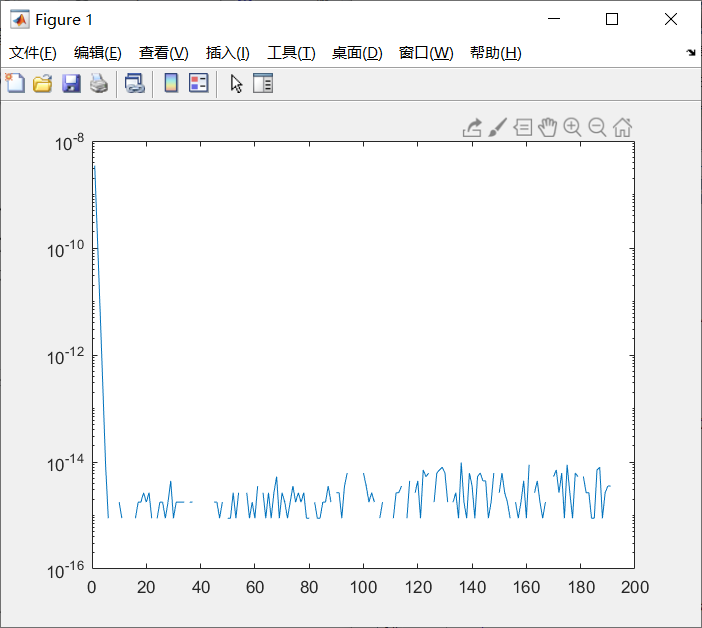
\includegraphics[width=0.8\textwidth]{3.png}
    	\caption{不同子区间数量下计算面积的误差图像}\label{jpg:3}
	\end{figure}

	\item[第三题] 
	(a)(10分)推导出如下格式的多步法公式:
$$y_{n+1}=y_{n-1}+\alpha f_{n+1}+\beta f_{n}+\gamma f_{n-1}$$

则积分区间为$[x_{n-1},x_{n+1}]$,积分节点为$\{x_{n+1},x_n,x_{n-1}\}$
$$y_{n+1}=y_{n-1}+h(a_0 f(x_{n+1},y_{n+1}),a_1 f(x_n,y_n),a_2 f(x_{n-1},y_{n-1}))$$
其中的积分系数为
$$\alpha=\int_{x_{n-1}}^{x_{n+1}}\frac{(x-x_n)(x-x_{n-1})}{(x_{n+1}-x_n)(x_{n+1}-x_{n-1})}dx=\frac 1 3 h$$
$$\beta=\int_{x_{n-1}}^{x_{n+1}}\frac{(x-x_{n+1})(x-x_{n-1})}{(x_{n}-x_{n+1})(x_{n}-x_{n-1})}dx=\frac 4 3 h$$
$$\gamma=\int_{x_{n-1}}^{x_{n+1}}\frac{(x-x_{n+1})(x-x_n)}{(x_{n-1}-x_{n+1})(x_{n-1}-x_{n})}dx=\frac 13 h$$
	即
$$y_{n+1}=y_{n-1}+\frac h3(f_{n+1}+4 f_{n}+ f_{n-1})$$


	(b) (10分)推导此格式的局部截断误差,并由此指明此格式的阶数。\\

将$$y_{n+1}=y_{n-1}+\frac h3(f_{n+1}+4 f_{n}+ f_{n-1})$$
在$x_n$处作 Taylor 展开,与$y(x_{n+1})$在$x_n$处的 Taylor 展开式做比较,即可
得到局部截断误差表达式
	$$T_{n+1}= \frac 13 h^3y^{(3)}(\eta)$$
	为2阶

	(c) (10分)选取合适的步长值,用此格式在$[0, 2]$上解如下的初值问题:
$$y^\prime=x e^{-4x}-4y, y(0)=0$$
使用你刚刚推导出的格式,并利用二阶Runge-Kutta方法(即课本公式(7.15))起步。画出解函数。\\

预估校正公式
$$y_{n+1}=y_{n-1}+\frac h3(7f_{n+1}-2 f_{n}+ f_{n-1})$$

	代码如下:\\
\begin{lstlisting}[frame=single,numbers=left]
clc,close

f = @(x, y) x * exp(-4 * x) - 4 * y;

n = 2000;
h = 2 / n;

x = zeros(1, n);
y = zeros(1, n);
k1 = f(0, 0);
k2 = f(h / 2, h / 2 * k1);
x(2) = h;
y(2) = y(1) + h * k2;
k1 = f(h, y(2));
k2 = f(x(2) + h / 2, y(2) + h / 2 * k1);
x(3) = x(2) + h;
y(3) = y(2) + h * k2;
f1 = f(x(1), y(1));
f2 = f(x(2), y(2));
f3 = f(x(3), y(3));
for i = 3 : n
    x(i + 1) = x(i) + h;
    tmp = (y(i - 1) + h * (7/3 * f3 - 2/3 * f2 + 1/3 * f1));
    y(i + 1) = (y(i - 1) + h * (1/3 * f(x(i + 1), tmp) + 4/3 * f3 + 1/3 * f2));
    f1 = f2;
    f3 = f(x(i + 1), y(i + 1));
end

plot(x, y)
\end{lstlisting}

得到的解函数如下图\ref{jpg:4}\\
	\begin{figure}[H]
		\centering
     	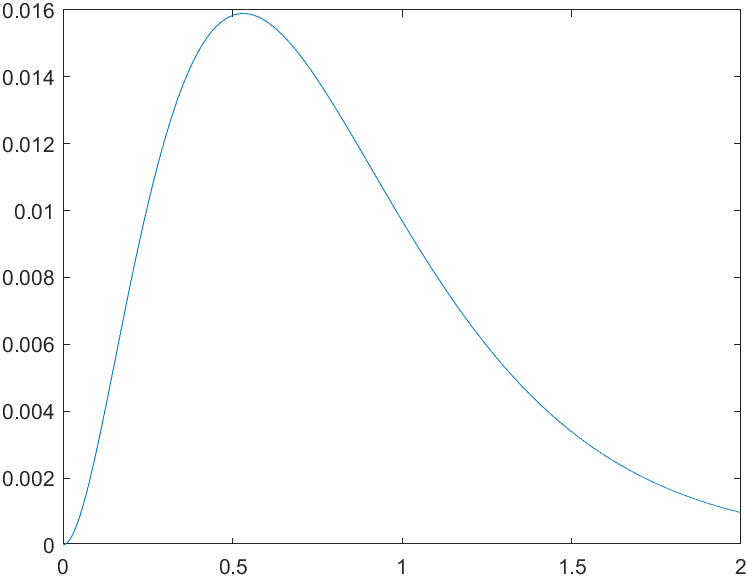
\includegraphics[width=0.8\textwidth]{4.png}
    	\caption{[0,2]的解函数图像}\label{jpg:4}
	\end{figure}


	(d) (10分)推导出(2)的精确解。对比该精确解在x = 2这一点的值,用log-log图
展示所用方法的阶数,并给出解释。\\

	观察得,可设$y = (ax^2+bx+c)e^{-4x}$,代入得
$$(-4ax^2+(2a-4b)x+b-4c)e^{-4x}=xe^{-4x}-4(ax^2+bx+c)e^{-4x}$$
对比系数可得到
$$\left\{
\begin{aligned}
-4a =-4a \\
2a-4b=1-4b\\
b-4c=-4c
\end{aligned}
\right.$$
则$a = \frac 12,b=0$,又由$y(0)=0$得c=0,代入得
$$y=\frac 12 x^2e^{-4x}$$

	代码如下:\\
\begin{lstlisting}[frame=single,numbers=left]
clc,close

f = @(x, y) x * exp(-4 * x) - 4 * y;
exc = 1/2 * 2^2 * exp(-4 * 2);
x0 = 10:10000;
z = zeros(1, length(x0));
for n = 10 : 10000
    h = 2 / n;
    x = zeros(1, n);
    y = zeros(1, n);
    k1 = f(0, 0);
    k2 = f(h / 2, h / 2 * k1);
    x(2) = h;
    y(2) = y(1) + h * k2;
    k1 = f(h, y(2));
    k2 = f(x(2) + h / 2, y(2) + h / 2 * k1);
    x(3) = x(2) + h;
    y(3) = y(2) + h * k2;
    f1 = f(x(1), y(1));
    f2 = f(x(2), y(2));
    f3 = f(x(3), y(3));
    for i = 3 : n
        x(i + 1) = x(i) + h;
        tmp = (y(i - 1) + h * (7/3 * f3 - 2/3 * f2 + 1/3 * f1));
        y(i + 1) = (y(i - 1) + h * (1/3 * f(x(i + 1), tmp) + 4/3 * f3 + 1/3 * f2));
        f1 = f2;
        f2 = f3;
        f3 = f(x(i + 1), y(i + 1));
    end
    z(n - 9) = abs(y(n + 1) - exc);
end

loglog(x0,z)
\end{lstlisting}

得到的loglog图像如下图\ref{jpg:5}\\
	\begin{figure}[H]
		\centering
     	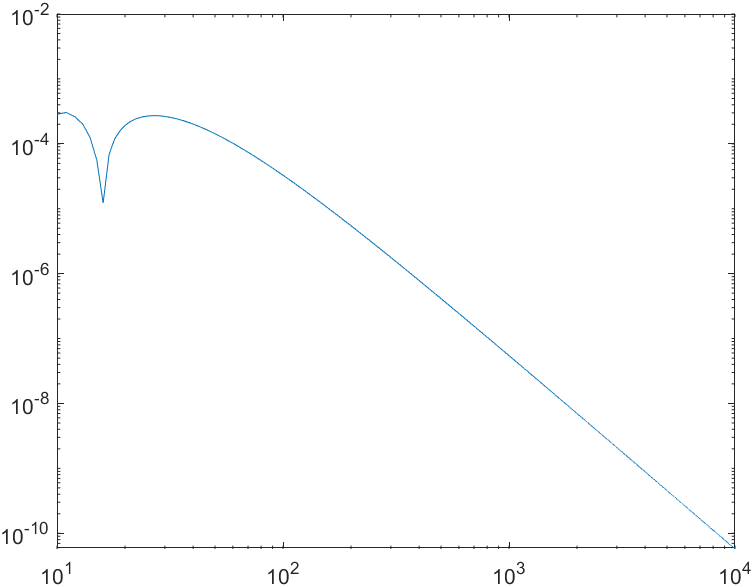
\includegraphics[width=0.8\textwidth]{5.png}
    	\caption{loglog图像}\label{jpg:5}
	\end{figure}
由图像知斜率约为3,阶数为3
\end{enumerate}
\end{document}